 \section{Durchführung}
\label{sec:Durchführung}
Bei allen drei Messreihen, zwei mit verschiedenen Einzelspalten, eine mit einem Doppelspalt, wird der Aufbau in Abbildung \ref{fig:experimentelleraufbau} auf einer optischen Schiene verwendet.
\begin{figure}[h!]
	\centering
	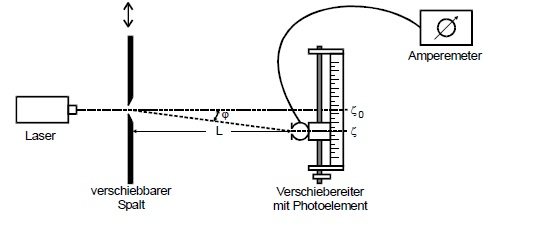
\includegraphics[width=0.9\linewidth]{experimentelleraufbau.jpg}
	\caption{Experimenteller Aufbau zur Ausmessung der Beugungsfigur, \cite[7]{anleitung406}.}
	\label{fig:experimentelleraufbau}
\end{figure}
Als Lichtquelle wird ein Helium-Neon-Laser mit einer Wellenlänge von $\SI{635}{\nano\metre}$ verwendet. Dieser wird auf einen Parallelspalt gerichtet, dessen Breite im Versuch bestimmt werden soll. Im Abstand von einem Meter befindet sich ein Photoelement auf einem Verschiebemessreiter. So kann das Beugungsbild schrittweise abgetastet werden. Die Intensität des gebeugten Lichts wird mit einer Photodiode gemessen, die einen zur Intensität proportionalen Strom erzeugt. Wichtig ist aufgrund der geringen entstehenden Stromstärken noch der Dunkelstrom, also der Strom, den die Photodiode ohne eingeschalteten Laser abgibt. Dieser wird dann von den Messergebnissen abgezogen.

Die Photodiode kann senkrecht zum ungebeugten Lichtstrahl auf einem Messreiter verschoben werden. Danach fängt die Messung für den ersten Einzelspalt an. Dabei muss auch noch der Dunkelstrom aufnotiert werden, da dieser bei der Auswertung des Messergebnisse wichtig ist. Die Messungen werden im Dunkeln durchgeführt. Der gemessene Photostrom wird an einem Amperemeter abgelesen und es wird auch der Abstand aufgeschrieben. 

Der Spalt und der Laser werden so ausgerichtet, dass die Beugungsfigur möglichst hell und parallel zum Photoelement verläuft. Um eine symmetrische Verteilung der Messwerte zu erreichen wird das Hauptmaximum so ausgerichtet, dass dieses gemessen wird, wenn sich die Photozelle auf der Mitte des Verschiebemessreiter befindet. Der Verschiebemessreiter kann über $\SI{50}{\milli\meter}$ verschoben werden, es werden 50 Messwerte je Beugungsfigur genommen. Zu den beiden Einzelspalten werden jeweils 50 Messwerte aufgenommen und bei dem Doppelspalt jeweils doppelt so viele als bei dem Einzelspalt.